\section{ACTIVIDAD 02 Creación de un Data Source View}

Si bien es cierto hemos creado una conexión hacia Adventure Works DW, solo trabajaremos con algunas tablas. 			Seleccionamos las tablas DimDate,DimProduct y FactInternetSales:
	\begin{center}
	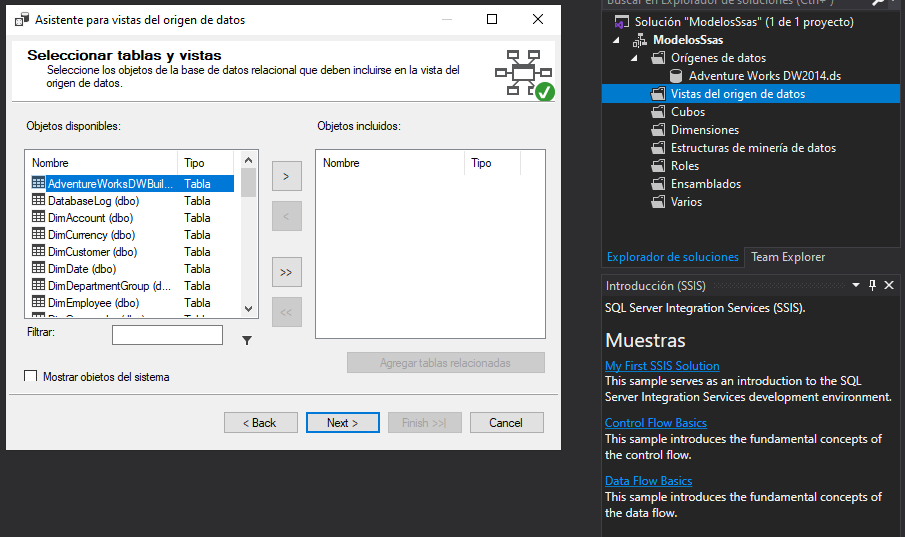
\includegraphics[width=\columnwidth]{images/task1/9}
    \end{center}	
    
Colocamos un nombre el Data Source View creado y click en Finish:
	\begin{center}
	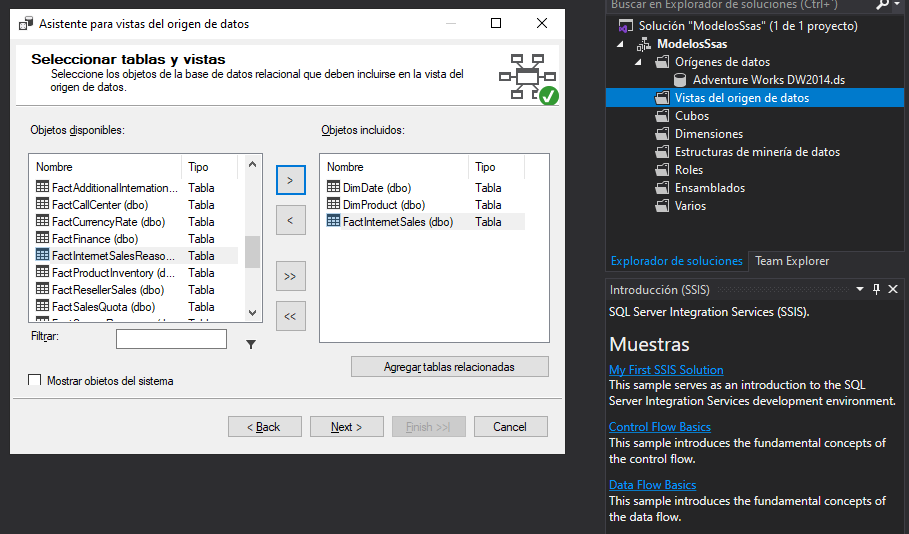
\includegraphics[width=\columnwidth]{images/task1/10}
    \end{center}	
    
	\begin{center}
	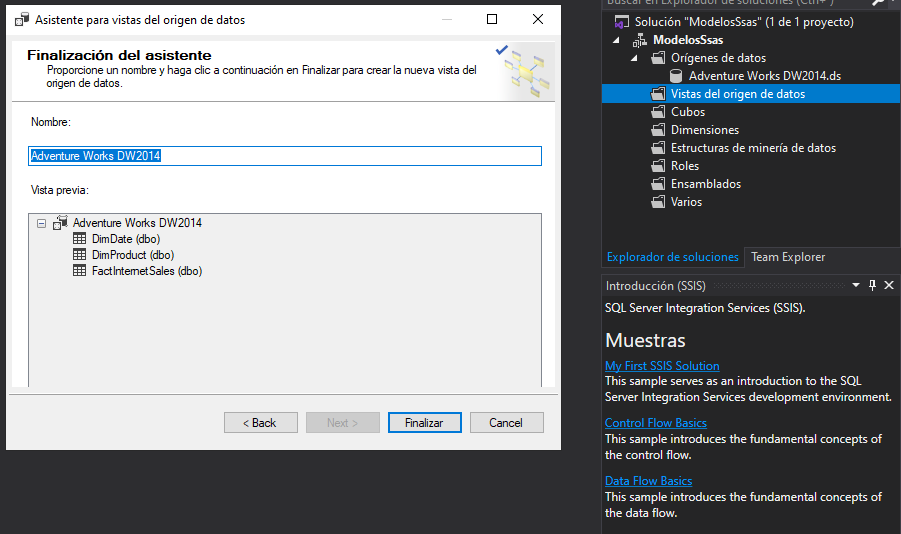
\includegraphics[width=\columnwidth]{images/task1/11}
    \end{center}	
    
Si todo va bien visualizaremos las tablas seleccionadas en el Data Source View:
	\begin{center}
	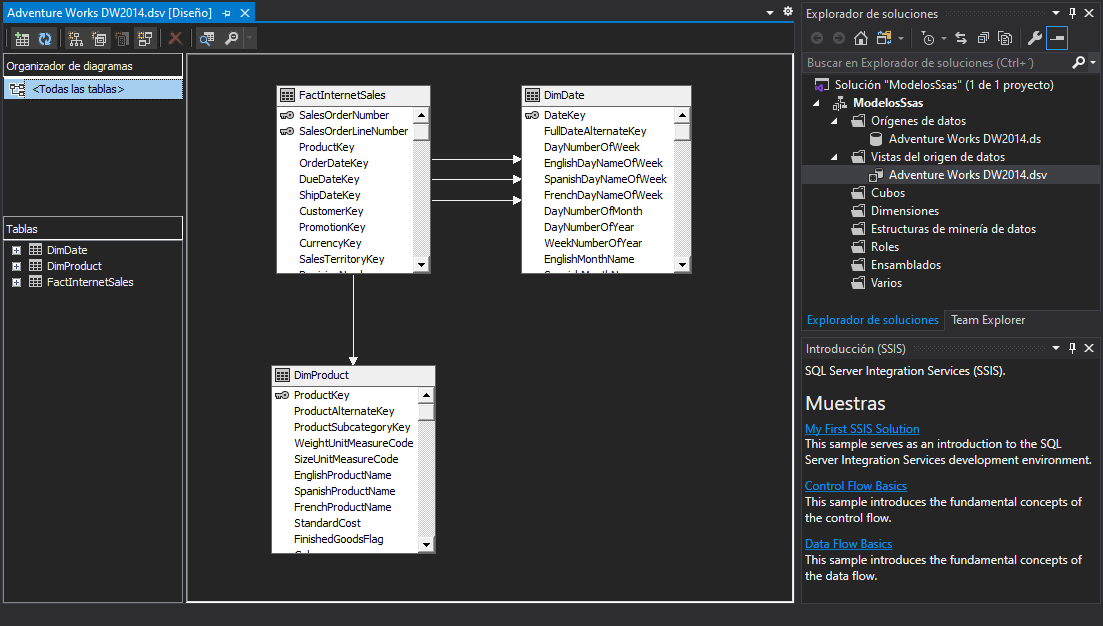
\includegraphics[width=\columnwidth]{images/task1/12}
	\end{center}	
	
\section{ACTIVIDAD 03 Creación de un Cubo}

En el Solution Explorer nos ubicamos en Cubes y click derecho, seleccionando la opción de New Cube
	\begin{center}
	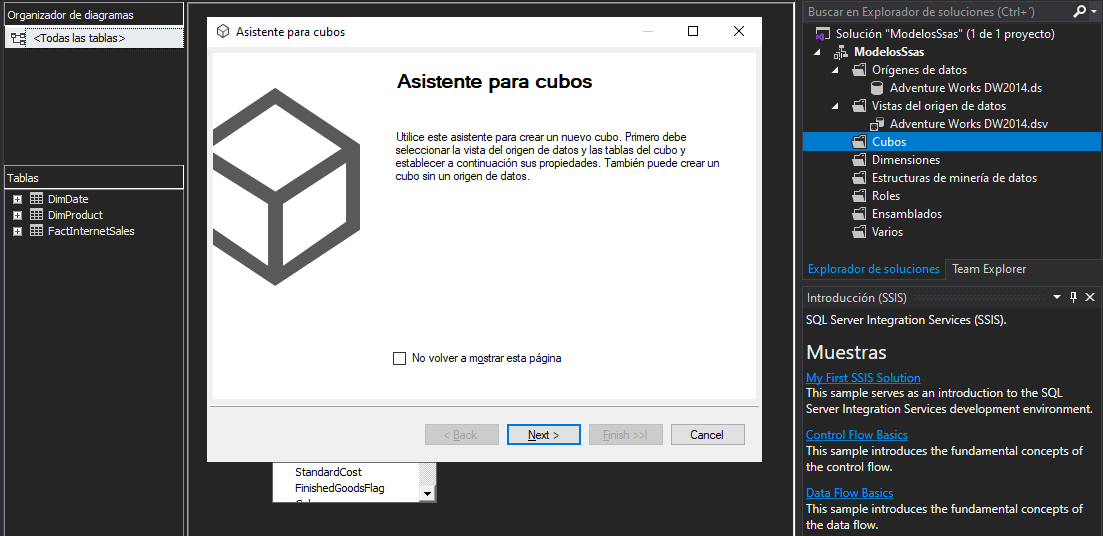
\includegraphics[width=\columnwidth]{images/task1/13}
    \end{center}	
    
Aquí seleccionaremos la FactTable (Tablas de Hechos) , en este caso ubicamos FactInternetSales
	\begin{center}
	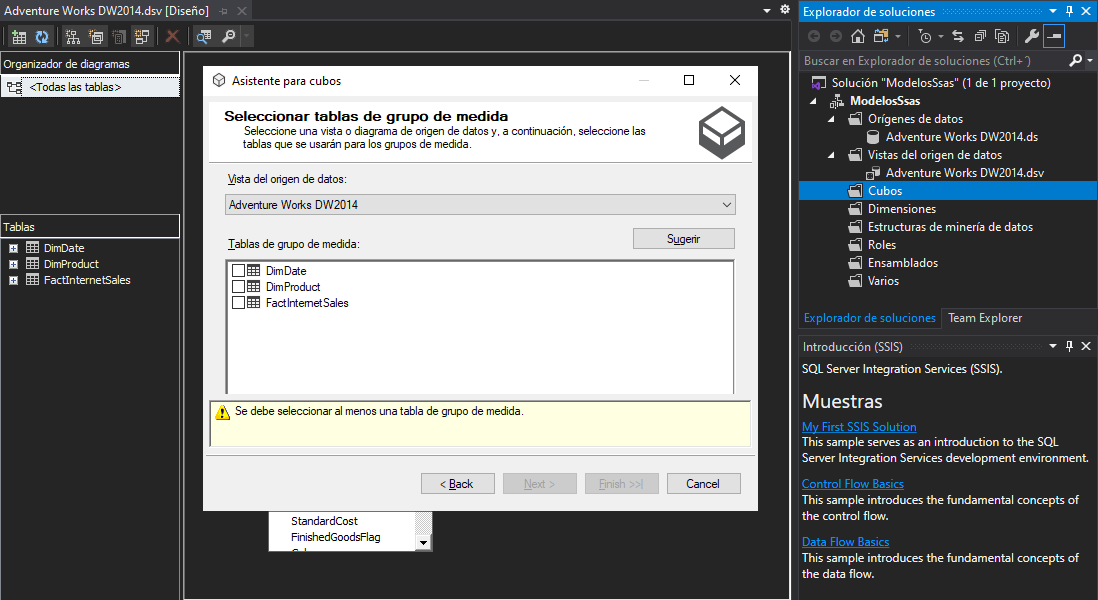
\includegraphics[width=\columnwidth]{images/task1/14}
    \end{center}	
    
Automáticamente el Data Tools identificará todos los campos numéricos y los marcará como candidatos a ser medidas. Podemos observar que inclusive marca los campos utilizados como Foregin Keys. En este caso, seleccionamos solo Order Quantity y Sales Amount:
	\begin{center}
	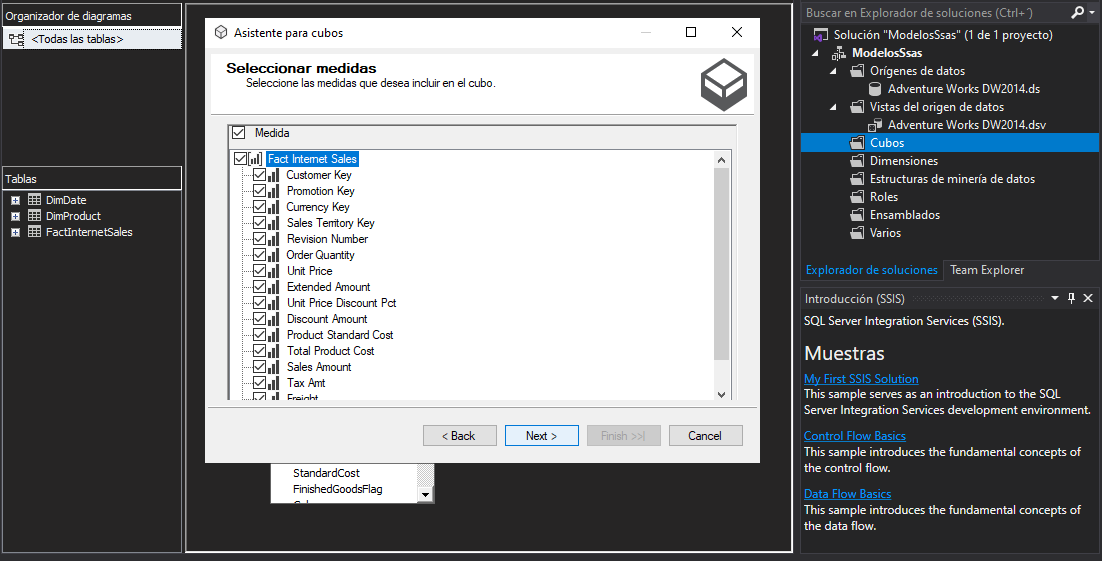
\includegraphics[width=\columnwidth]{images/task1/15}
    \end{center}	
    
Aquí seleccionamos las dimensiones por las cuales será analizada la data. Inclusive el Data Tools te indica que podría tomar la misma FactTable como Dimensión. Seleccionamos Dim Date y Dim Product:
	\begin{center}
	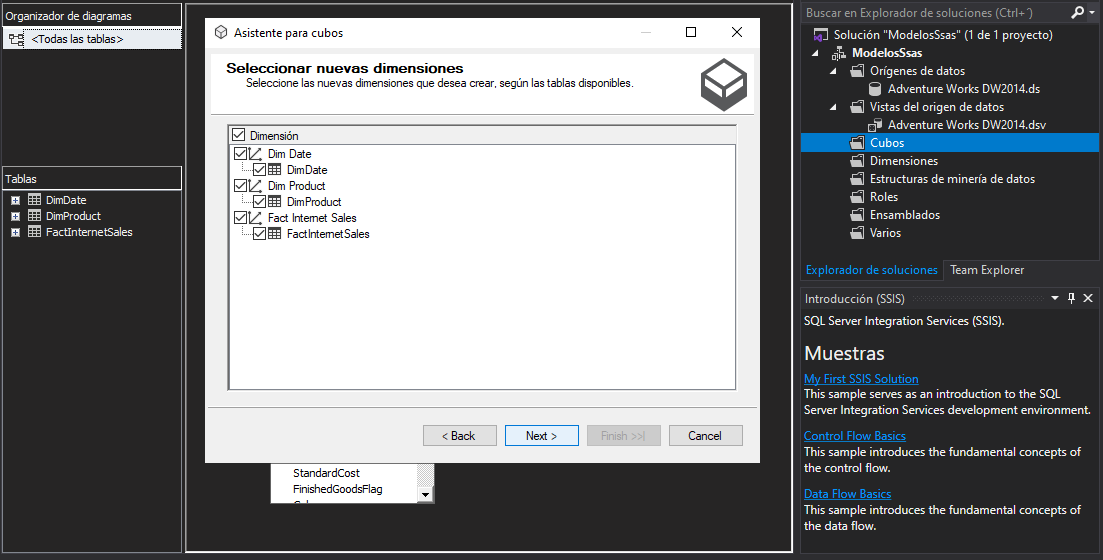
\includegraphics[width=\columnwidth]{images/task1/16}
	\end{center}	

Colocamos un nombre el cubo:
	\begin{center}
	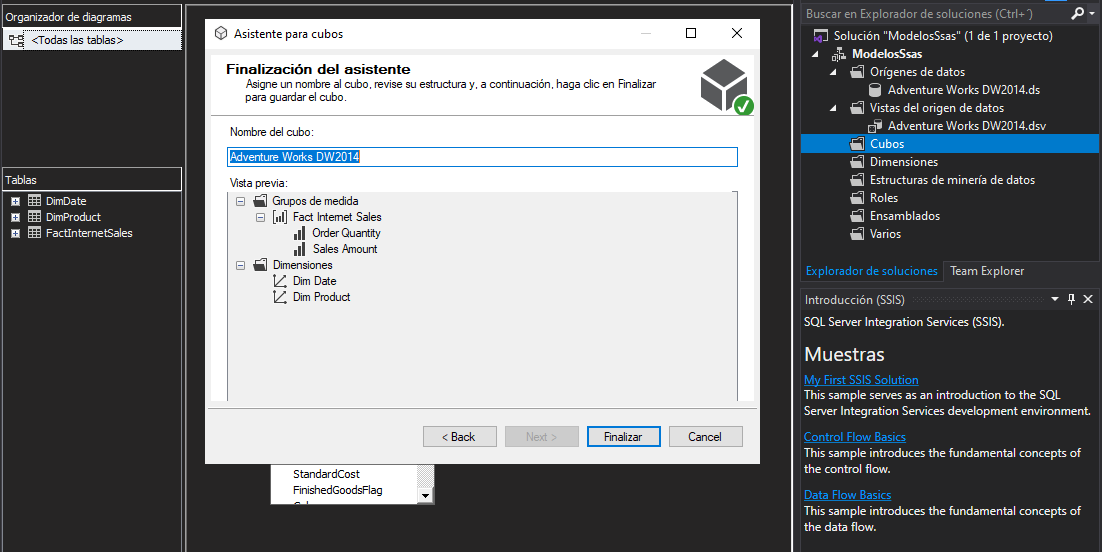
\includegraphics[width=\columnwidth]{images/task1/17}
	\end{center}	
	
En el Solution Explorer nos ubicamos en el nuevo cubo creado CubeSales y click derecho, seleccionando la opción de Process
		\begin{center}
	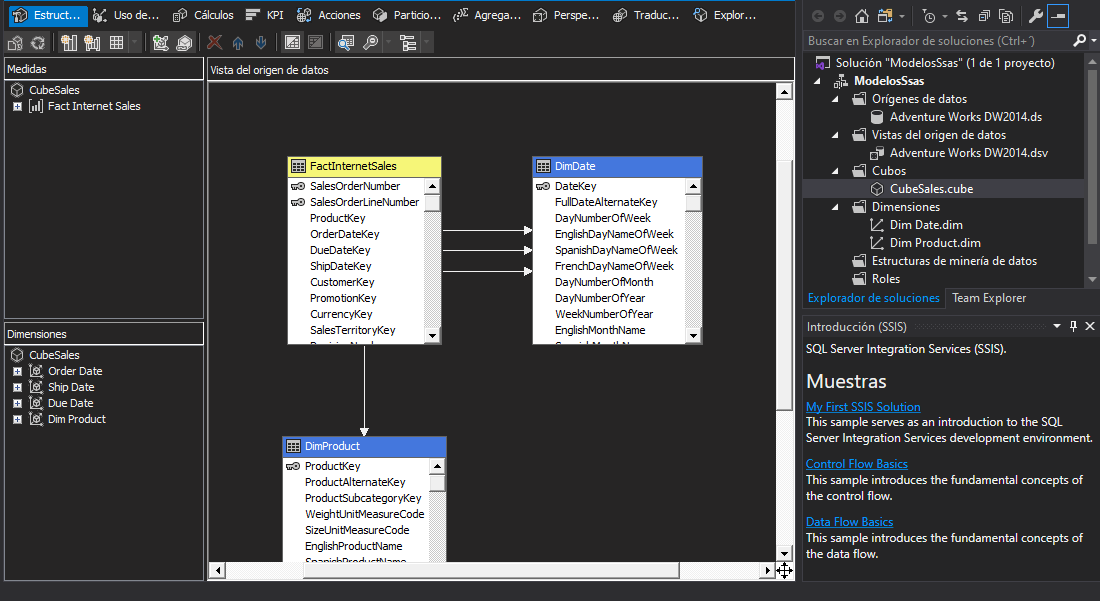
\includegraphics[width=\columnwidth]{images/task1/18}
	\end{center}	
	

	
